
\subsubsection{Алгоритмы работы с батиметрией}

Казалось бы, что тут сложного?
Обычная растровая модель высот, к тому же совмещенная с рельефом суши, а значит в ней отсутствуют пустые ячейки без значений.

Но чего в ней полно, так это погрешностей определения высотных и батиметрических отметок вдоль береговой линии, что можно увидеть на рисунке~\ref{pic:NVRSK_EMODnet_coastline_errors}.

\begin{figure}
    \begin{center}
	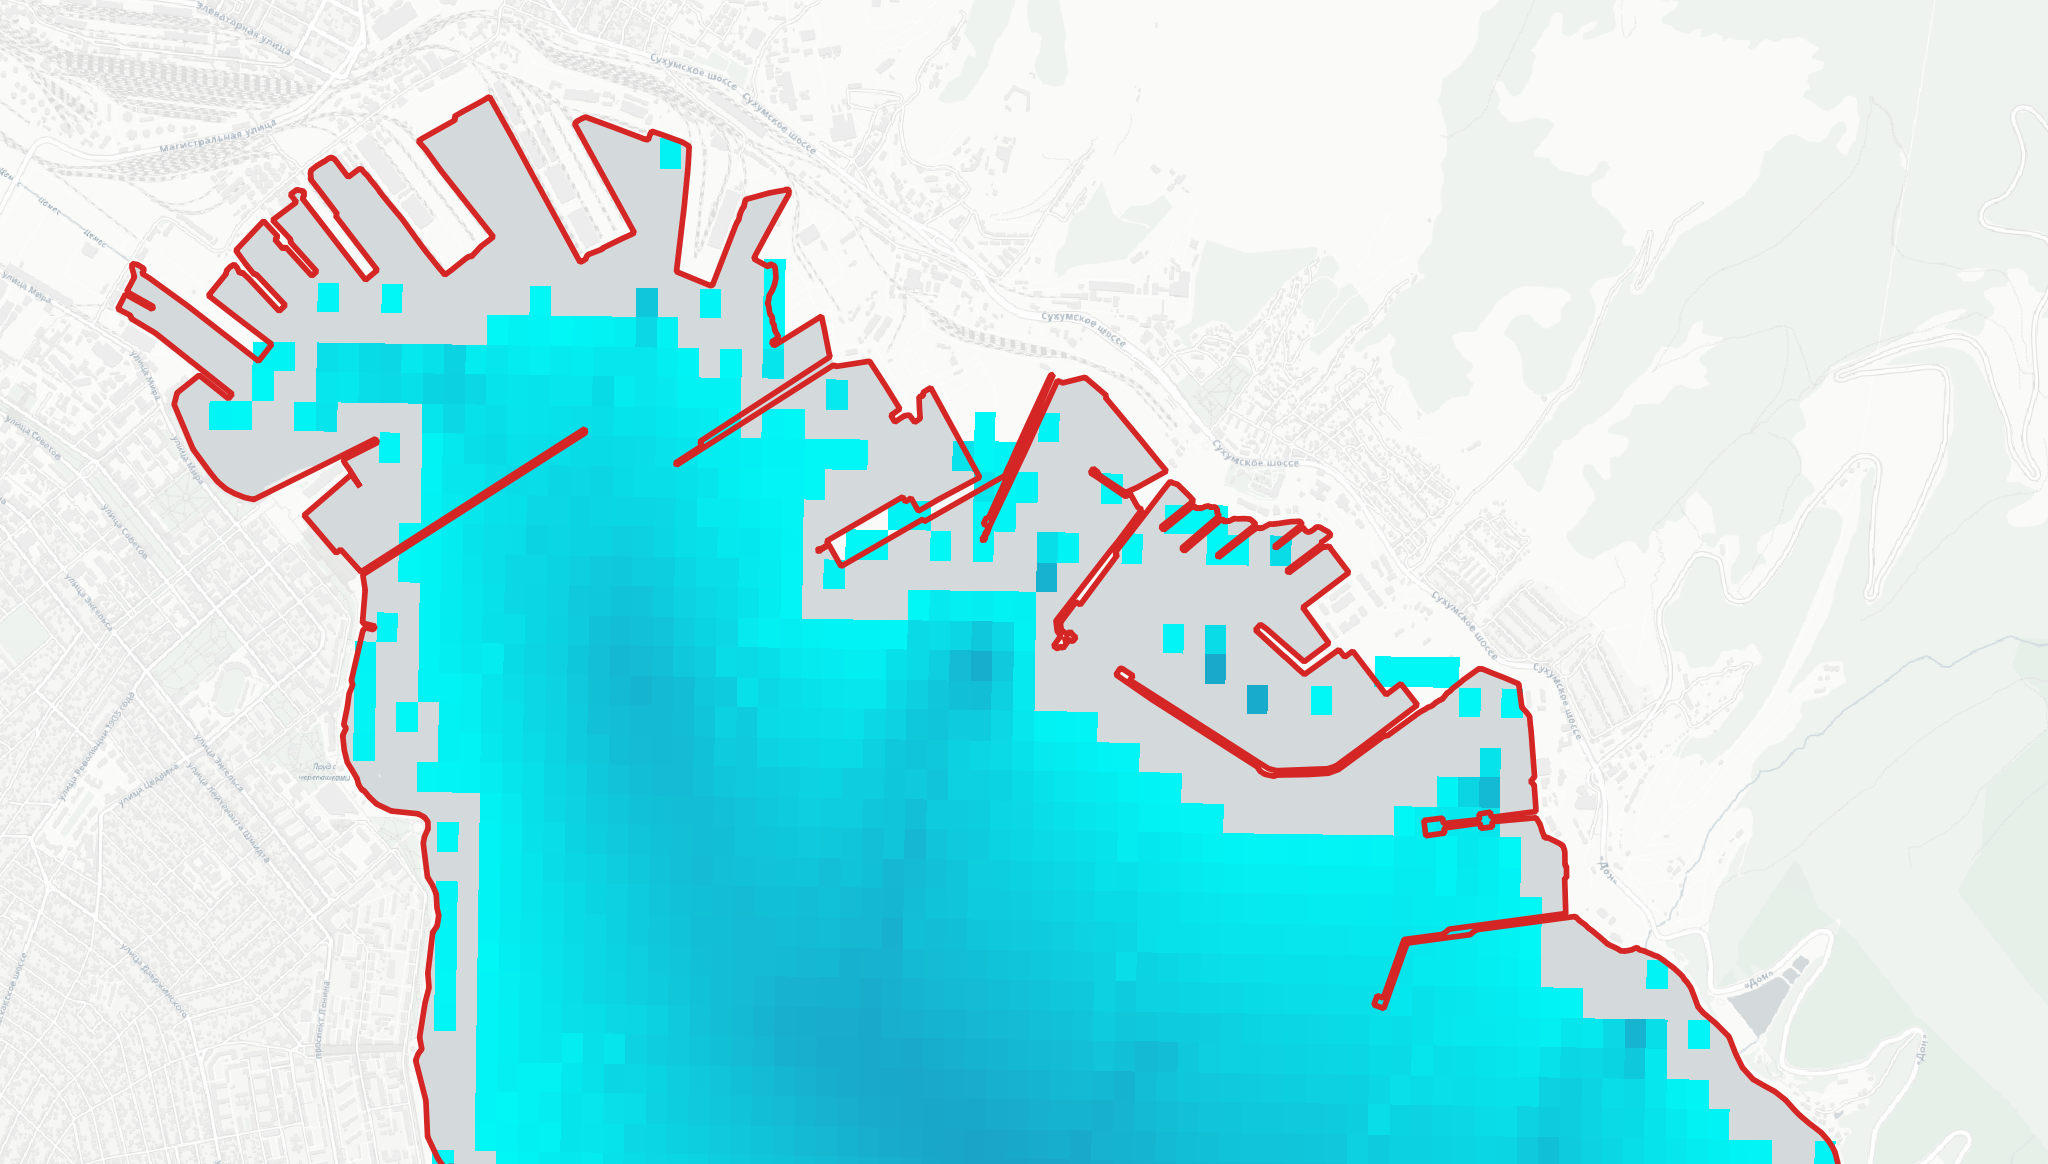
\includegraphics[width=120mm]{fig/part_2/alghoritm/NVRSK_EMODnet_coastline_errors.png}
	\caption{-- Демонстрация отсутствия данных батиметрии вдоль береговой линии в модели EMODnet}
	\label{pic:NVRSK_EMODnet_coastline_errors}
    \end{center}
\end{figure}

Ожидать иного от глобальной топографической модели, сформированной из множества рассогласованных по точности и времени источников данных было бы наивно.

Но делать нечего -- в базовом варианте ничего другого у нас нет.
Необходимость корректировки параметров волн при шоалинге и рефракции требует построения профиля морского дна вдоль направления движения волны и определения минимальной глубины вдоль берега. 

Для каждой прибрежной точки строится трансект от этой точки на определенное расстояние \texttt{radius\_m} по шагам \texttt{n\_steps}.
Вдоль трансекта из GeoTIFF-растра считываются значения глубины, получаемые путем интерполяции между смежными ячейками модели.
В целях минимизации повторяющихся вычислений каждый построенный профиль кэшируется и возвращается в случае повторного запроса для точки вдоль рассматриваемого направления.

После чего глубина $h_{deep}$ выбирается как максимальная валидная глубина вдоль профиля -- характерная глубина для этой линии на открытой воде.
Глубина $h_{point}$ выбирается как первая валидная глубина у берега: либо первый элемент профиля с положительной глубинойй, либо первая валидная точка в массиве (в случае если профиль не пересекает батиметрические данные). 
Далее это глубина принимается как глубина непосредственно у рассматриваемой точки берега.

На том же профиле глубин модель выполняется поиск первой от берега глубины удовлетворяющей условию $H_s \ge \gamma_b h$.
Итоговая высота прибрежной волны берется как минимум из высоты после осушения и высоты при обрушении ($\min(H_{s,\text{shoaled}}, H_{s,\text{break}})$).
Параллельно, по $h_{deep}$, $h_{point}$ и периоду $T_p$ модель рефракции решает дисперсионное уравнение, вычисляет фазовые скорости на глубине и у берега и применяет закон Снеллиуса, возвращая косинус рефракции и угол преломления волны.

Оценивая качество батиметрических данных, следует признать, что именно они являются наиболее слабым местом рассматриваемой методики.
Хотя в разработанной программе нет технических препятствий к использованию внешних, более качественных, батиметрических съемок фактическое их отсутствие не дает возможность оценить степень влияния погрешностей в открытых данных на результат.

При выполнении расчетов в работе были рассмотрены варианты замены непосредственно определяемых из батиметрии глубин некоторыми обобщающими константами, но во всех случаях результат оказался неудовлетворительным.
В результате можно сделать вывод -- даже самая плохая батиметрия многократно лучше, чем ее отсутствие.

\subsection{Выводы по разделу} 

В предыдущих параграфах текущего раздела были описаны частные вопросы и решения реализации методики расчета волновой нагрузки на берег.
Приведенных в них алгоритмов достаточно, чтобы выполнить все необходимые расчеты, описанные в разделе~\ref{part:sea_stuff}.
Не без трудностей и вычислительных компромиссов это было реализовано в виде программного продукта, доступного в репозитории, ссылка на который представлена на рисунке~\ref{pic:BreachTheBeach_qr_code}.

\begin{figure}
    \begin{center}
	
\includegraphics[width=60mm]{fig/part_2/BreachTheBeach_qr_code.png}
	\caption{-- QR код на страницу репозитория проекта}
	\label{pic:BreachTheBeach_qr_code}
    \end{center}
\end{figure}
